\documentclass[border=20pt]{standalone}
\usepackage[utf8]{inputenc}
\usepackage{tikz}
\usetikzlibrary{arrows.meta, chains, positioning}
\usepackage{amssymb}

\begin{document}
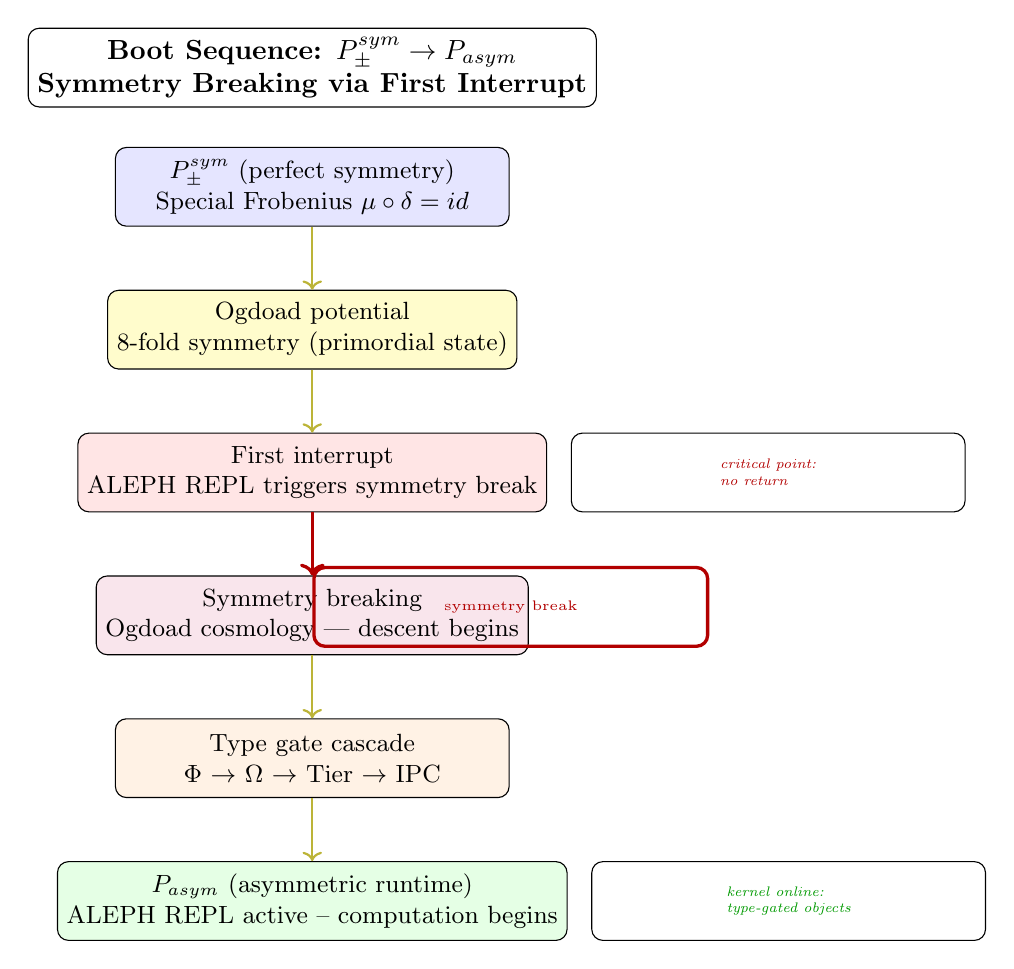
\begin{tikzpicture}[
  start chain=going below,
  node distance=0.8cm,
  every node/.style={on chain, draw, rounded corners, minimum width=5cm, minimum height=1cm, align=center, font=\small}
]
  \node[fill=blue!10] (s1) {$P_{\pm}^{\text{sym}}$ (perfect symmetry)\\Special Frobenius $\mu \circ \delta = \text{id}$};
  \node[fill=yellow!20] (s2) {Ogdoad potential\\8-fold symmetry (primordial state)};
  \node[fill=red!10] (s3) {First interrupt\\ALEPH REPL triggers symmetry break};
  \node[fill=purple!10] (s4) {Symmetry breaking\\Ogdoad cosmology --- descent begins};
  \node[fill=orange!10] (s5) {Type gate cascade\\$\Phi$ $\to$ $\Omega$ $\to$ Tier $\to$ IPC};
  \node[fill=green!10] (s6) {$P_{\text{asym}}$ (asymmetric runtime)\\ALEPH REPL active -- computation begins};

  % Arrows
  \draw[->, thick, yellow!70!black] (s1) -- (s2);
  \draw[->, thick, yellow!70!black] (s2) -- (s3);
  \draw[->, thick, red!70!black, line width=1.2pt] (s3) -- (s4) node[midway, right, font=\tiny] {symmetry break};
  \draw[->, thick, yellow!70!black] (s4) -- (s5);
  \draw[->, thick, yellow!70!black] (s5) -- (s6);

  % Side annotations
  \node[right=0.3cm of s3, align=left, font=\tiny\itshape, text=red!70!black] {critical point:\\no return};
  \node[right=0.3cm of s6, align=left, font=\tiny\itshape, text=green!60!black] {kernel online:\\type-gated objects};

  % Title
  \node[above=0.5cm of s1, font=\bfseries, align=center] {Boot Sequence: $P_{\pm}^{\text{sym}} \to P_{\text{asym}}$\\Symmetry Breaking via First Interrupt};
\end{tikzpicture}
\end{document}
